\documentclass
[
a4paper,
german,
openright,                    % Kap.beginn immer rechts! (fkt. nur bei report, nicht bei article)
12pt                          % ersatzweise 12pt, wenn mehr Seiten entstehen sollen
]
{report}
%%%%%%%%%%%%%%%%%%%%%%%%%%%%%%%%%%%%%%%%%%%%%%%%%%%%%%%%%%%%%%%%%%%%%%%%%%%%%%%%%%%%%%%%%%%%%%%%%%%%%%%%%%%%
%Dokumenteneigenschaften

\newcommand{\Author}{Refik Kerimi} 
\newcommand{\Title}{Analyse der Auswirkung von Progressive Web Apps auf bestehende Apps}
\newcommand{\Keywords}{Progressive Web App, mobile App, native App, Android, ios}
\newcommand{\Advisor}{DI Norbert Egger BSc}
\newcommand{\Birthdate}{28.03.1983}
\newcommand{\EnrolNum}{1410555043}
\newcommand{\VenueMonthYear}{Salzburg, September 2018}
\newcommand{\VenueDate}{Salzburg, am 1.09.2018}

\newcommand{\frontmatter}{\cleardoublepage\pagenumbering{roman}}

\newcommand{\mainmatter}{\cleardoublepage\pagenumbering{arabic}\setcounter{page}{1}}

%%%%%%%%%%%%%%%%%%%%%%%%%%%%%%%%%%%%%%%%%%%%%%%%%%%%%%%%%%%%%%%%%%%%%%%%%%%%%%%%%%%%%%%%%%%%%%%%%%%%%%%%%%%%
% Layout zusammengestellt von Richard Wanger im WS 2015/2016. Verschiedene Vorlagen wurden bei der Erstellung
% kombiniert und nach dem Masterleitfaden (Stand: Oktober 2015) adaptiert. Verwendung ohne Gewähr!
% Umbau des Layouts nach dem Bachelorleitfaden (Stand: Juni 2018) durch Refik Kerimi SS 2018 

\usepackage{style}		%alle packages und Formatvorlagen befinden sich in dieser Datei


%%%%%%%%%%%%%%%%%%%%%%%%%%%%%%%%%%%%%%%%%%%%%%%%%%%%%%%%%%%%%%%%%%%%%%%%%%%%%%%%%%%%%%%%%%%%%%%%%%%%%%%%%%%%
% ORGANISATORISCHES

\usepackage{amsmath}
\usepackage{amsfonts}
\usepackage{amssymb}


\begin{document}

\begin{titlepage}

\hspace{7cm}

\begin{center}
	{\Large\uppercase\expandafter{\bf BACHELORARBEIT}}\\[0.5ex]
	\vspace{1cm}
	\Large{\bf\large \Title}\\
	\vspace{1.5cm}
	\normalsize durchgeführt am\\
	Studiengang Informationstechnik \& System--Management\\
	an der\\
	Fachhochschule Salzburg GmbH\\
\end{center}

\vspace{2cm}

\begin{center}
	\normalsize vorgelegt von
	\\
	{
		\Large{\bf\large \Author}\\
	}
	\vspace{2cm}
	
\includegraphics[width=7cm]{BilderAllgemein/Logo.jpg}\medskip
\end{center}
	
\vspace{2cm}

\begin{tabbing}
	\hspace*{3cm}\=\hspace*{4cm}\= \kill
	\> Studiengangsleiter: \> FH-Prof.~DI Dr. Gerhard Jöchtl \\*[0.2cm]
	\> Betreuer: \> \Advisor
\end{tabbing}

\vfill	

\begin{center}
\VenueMonthYear\\
\end{center}
\end{titlepage}
\chapter*{Eidesstattliche Erklärung}
\thispagestyle{plain}
\pagestyle{plain}

Ich versicheren an Eides statt, dass ich die vorliegende Bachelorarbeit ohne unzulässige fremde Hilfe und ohne Benutzung anderer als der angegebenen Quellen und Hilfsmittel angefertigt und alle aus ungedruckten Quellen, gedruckter Literatur oder aus dem Internet im Wortlaut oder im wesentlichen Inhalt übernommenen Formulierungen und Konzepte gemäß den Richtlinien wissenschaftlicher Arbeiten zitiert, bzw. mit genauer Quellenangabe kenntlich gemacht habe. Diese Arbeit wurde in gleicher oder ähnlicher Form weder im In- noch im Ausland in irgendeiner Form als Prüfungsarbeit vorgelegt und stimmt mit der durch die Begutachter beurteilten Arbeit überein.
\vspace{3cm}

\VenueDate

\vspace{0.5cm}

\begin{tabular}{p{0.3\textwidth}p{0.32\textwidth}p{0.3\textwidth}}



\parbox[c]{1em}{
\includegraphics[width=5cm]{BilderAllgemein/unterschriftRef.jpg}} &  &  \multicolumn{1}{c}{1410555043} \\ \cline{1-1} \cline{3-3}

Refik Kerimi & & Matrikelnummer


\end{tabular}
\chapter*{Allgemeine Informationen}
\thispagestyle{plain}
\pagestyle{plain}
\renewcommand{\footrulewidth}{0.4pt}
\lfoot{\small Refik Kerimi}

\begin{tabular}{p{0.3\textwidth}p{0.65\textwidth}}

Vor- und Zuname: & \Author \\*[0.2cm]
Institution: & Fachhochschule Salzburg GmbH \\*[0.2cm]
Studiengang: & Informationstechnik \& System-Management \\*[0.2cm]
Titel der Masterarbeit: & \Title \\*[0.2cm]
Schlagwörter: & \Keywords  \\*[0.2cm]
Betreuer an der FH: & \Advisor

\end{tabular}

\newpage

\section*{\Large\bfseries Kurzfassung}
Die steigende Anzahl der von Mobilen Geräten erfordert ein umdenken in der Art der Applikationsentwicklung. 

Die steigenden Anforderungen an moderne Energiesysteme setzen eine Weiterentwicklung der Kommunikations- und Informationsinfrastruktur voraus. Das Ziel ist es, erneuerbare Energiequellen einfacher und effizienter in bestehende Netze zu integrieren.
Das Projekt OpenNES, welches gemeinsam vom \ac{AIT}, der FH Salzburg und der Fronius International GmbH entwickelt wird, soll eine offene, generische und interoperabe Informations- und Automatisierungslösung schaffen, die dies ermöglicht.
OpenNES stellt fern-programmierbare Funktionen, geeignete Modellierungsmethoden für Energiequellen und eine Infrastruktur zur Schaffung der Kommunikation bereit.
Zur Implementierung von nicht OpenNES fähigen Geräten in Smart Grids werden mehrere Protokolladapter benötigt. Diese befinden sich im Connectivity Modul, welches die Schnittstelle zur Kommunikation nach außen darstellt. 
In dieser Bachelorarbeit wird der Protokolladapter für Modbus/SunSpec entwickelt.
OpenNES soll dazu beitragen, dass die geforderten Ziele und Richtlinien der EU für Klimaschutz und Energie in Zukunft erreicht werden können.


\section*{\Large\bfseries Abstract}

Increasing requirements on modern energy systems require  further development of  communication and information infrastructure. The aim is to integrate renewable energy sources more easily and efficiently into existing networks. 
To ensure this, the project OpenNES, which is beeing developed jointly by the Austrian Intitute of Technology (ATI), the FH Salzburg and Fronius International GmbH, shall  create an open, generic and interoperable information and automation solution. 
OpenNES provides remote programmable features, appropriate modelling methods for energy sources, and an infrastructure to provide communication. 
Several protocol adapters are required to implement non-OpenNES-enabled devices in SmartGrids. These are located within the Connectivity Module, an interface for communication to the outside. 
In this bachelor thesis, the protocol adapter for Modbus/SunSpec is developed. 
OpenNES is intended to help achieve the EU's objectives and directives for climate protection and energy in the near future. 

\chapter*{Danksagung}
\thispagestyle{plain}
\pagestyle{plain}

Danken möchte ich vor allem meinem Betreuer für die Unterstützung bei dieser Bachelorarbeit. 

Besonderer Dank gilt auch meiner Familie und Freunden, die uns während des Studiums in allen Belangen immer unterstützt haben. 



































%%%%%%%%%%%%%%%%%%%%%%%%%%%%%%%%%%%%%%%%%%%%%%%%%%%%%%%%%%%%%%%%%%%%%%%%%%%%%%%%%%%%%%%%%%%%%%%%%%%%%%%%%%%%
%VERZEICHNISSE

\tableofcontents
%\protect\addcontentsline {toc}{chapter} {Inhaltsverzeichnis}

\frontmatter
\renewcommand{\nomname}{Abkürzungsverzeichnis}
\chapter*{Abkürzungsverzeichnis}
\addcontentsline{toc}{chapter}{Abkürzungsverzeichnis} 
\pagestyle{plain}

\begin{acronym}[AUTOSAR]

 \acro {PWA}  				{Progressive Web Applikationen}
 \acro {API} 				{Application Programming Interface}
 \acro {JS} 				{Java Script}
 \acro {IDE} 				{Entwicklungsumgebung}
 \acro {SHP} 				{Smart Home Prototypen}
 \acro {NA} 				{Nativen Applikation}
 \acro {MA} 				{Mobile Applikationen}
 \acro {WA}					{Web Applikationen}
 \acro {HTML5}				{Hypertext Markup Language}
 \acro {CSS}				{Cascading Style Sheets}
 \acro {HyApp}				{Hybrid Applikationen}
 \acro {SW}					{Service Worker}
 \acro {SC}					{Server-Client}
\end{acronym} 

\listoffigures
\protect \addcontentsline {toc}{chapter}{Abbildungsverzeichnis}

\listoftables
\protect \addcontentsline{toc}{chapter}{Tabellenverzeichnis}

\lstlistoflistings
\protect \addcontentsline{toc}{chapter}{Listingverzeichnis}

%%%%%%%%%%%%%%%%%%%%%%%%%%%%%%%%%%%%%%%%%%%%%%%%%%%%%%%%%%%%%%%%%%%%%%%%%%%%%%%%%%%%%%%%%%%%%%%%%%%%%%%%%%%%
%INHALT

\mainmatter
\chapter{Einleitung}

\thispagestyle{standard}
\pagestyle{standard}
\section{Motivation}



\section{Zielsetzung}


\section{Anmerkung}













\chapter{Grundlagen}
\thispagestyle{standard}
\pagestyle{standard}
\renewcommand{\footrulewidth}{0.4pt}
\lfoot{\small Refik Kerimi}

Wie in Kapitel \ref{chap:Einleitung} beschrieben, hat der stetige Zuwachs von \acl{SP}s \acs{SP}s \cite{Geraetenutzung} zum Umdenken bei der Planung und beim Entwickeln von Webapplikationen geführt.
Zu Beginn jedes Projektes steht die Entscheidung an, welche Technologien und Tools zur Entwicklung verwendet werden sollen um die bestmöglichen Ergebnisse zu erhalten.
Wenn die falschen Methoden gewählt werden, kann das zu gravierenden Fehlern in der Applikation führen, die sich erst mit Fortdauer der produktiven Verwendung ersichtlich machen. 
Die Frage ist, ob man sich für eine Anwendung die auf das Betriebssystem zugeschnitten ist oder doch für eine plattformübergreifende Webanwendung entscheidet. Beide Methoden haben Vorteile und Nachteile und werden im Zuge dieser Arbeit betrachtet. Den Kern der Arbeit aber stellten, die von Google entwickelten \acs{PWA} \cite{PWA} da. \\Die \acs{PWA}s sollen den Spagat zwischen diesen beiden Anwendungen schaffen. Eventuell könnte diese neue Form der Appentwicklung die traditionelle Technologien gar zur Gänze ablösen?
Der Trend der letzten Jahren geht in Richtung der mobilen Nutzung und da ist das \acl{SP} klar wie, in Abbildung \ref{fig:Internetnutzung} und \ref{fig:Smartphonenutzung} dargestellt, voran.  

\begin{figure}[h]
	\centering
	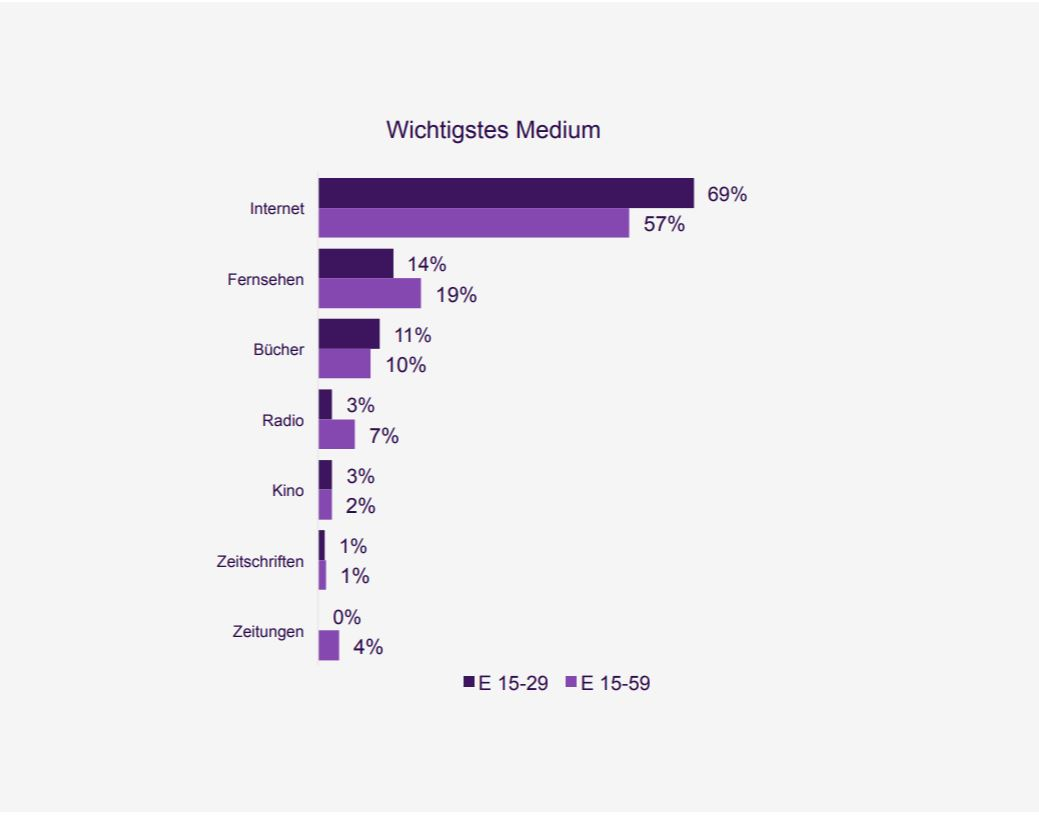
\includegraphics[width=6cm]{BilderAllgemein/Internetnutzung}\medskip
	\caption{Internetnutzung \cite{Geraetenutzung}}
	\label{fig:Internetnutzung}
\end{figure}

\begin{figure}[h]
	\centering
	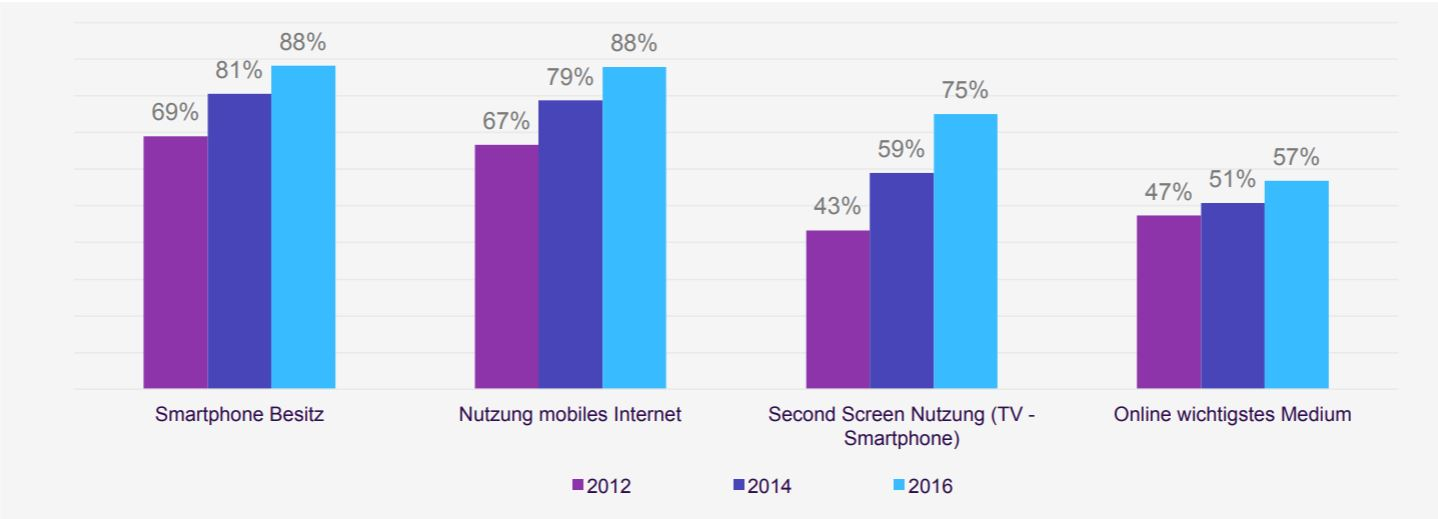
\includegraphics[width=8cm]{BilderAllgemein/SmartPhoneNutzung}\medskip
	\caption{Smartphonenutzung \cite{Geraetenutzung}}
	\label{fig:Smartphonenutzung}
\end{figure}

\section{Geschichte Softwareentwicklung}
Um die Geschichte der Softwareentwicklung darstellen zu können, müssen wir als aller erstes die Frage stellen "Was ist Software?" und wie ist eine Software definiert?
Diese Frage stellen sich sicherlich alle mal die zum ersten Mal in ihrem Leben mit dieser Technologie in Berührung kommen. Eine genau Definition zu finden ist schwierig da die Software für die Gesamtheit eines Produktes steht . In \cite{WasistSoftware} ist die Softwaretechnik wie folgt definiert:
\begin{quote}
\glqq Zielorientierte Bereitstellung und systematische Verwendung von Prinzipien, Methoden und Werkzeugen für
die arbeitsteilige, ingenieurmäßige Entwicklung und Anwendung
von umfangreichen Softwaresystemen. Zielorientiert bedeutet die
Berücksichtigung z.B. von Kosten, Zeit, Qualität.\grqq (\cite{WasistSoftware} Seite 17).
\end{quote}
Im Laufe der Jahre wurden verschiedenste Softwaren entwickelt, die mehr oder weniger nützlich für unseren Alltag waren.
Der Begriff Software wurde 1958 vom US-amerikanischen Statistiker John W. Turkey eingeführt.
Zu Beginn bildeten Software und Hardware eine Einheit. Erst nach der Entscheidung durch die US Regierung, dass IBM die Hardware und die Software separat verrechnen sollte, wurden sie getrennt.
Die Software bildet das Gehirn eines Computers. 
Nach der Entscheidung der US-Regierung entstanden erstmals rein softwareorienttiere Unternehmen wie Microsoft oder SAP \cite{Microsoft} \cite{SAP}. 


\section{Mobile Applikationen}
Anfang des neuen Jahrtausends war die Vorstellung, dass das Mobiltelefon für uns sehr viele alltäglichen Aufgaben erledigt unvorstellbar, doch heute können wir uns das Leben ohne 
Mobiltelefon kaum vorstellen.
Wir organisieren unser Leben damit und steuern unsere Haushaltsgeräte, unser Garagentor, verbinden uns mit unserem Auto usw. All diese Möglichkeiten werden durch Apps ermöglicht.
Die Apps werden im Allgemeinen in 3 Kategorien aufgeteilt
Native-, Web- und Hybridapps. 

\subsection{Native Apps}\label{chap:Native Apps}
\acl{NA}s (NA) (deutsch; angepasste Anwendung) sind speziell für eine Plattform angepasste Anwendungen. 
Diese werden speziell für ein bestimmtes Betriebssystem konzipiert und haben in der Regel Zugriff auf alle Ressourcen eines Gerätes \cite{NativeApp}.
Hauptsächlich werden zur Programmierung für Mobile Geräte die Hochsprachen Java (Android) und Swift(IOS) verwendet. Native Apps können in App Stores heruntergeladen  werden. \\Die bekanntesten sind Apple Store und Google Play \cite{Hochsprachen}.

\subsection{Web Applikationen}\label{chap:Webapplikationen}
Im Gegensatz zu den \acs{NA}s sind \acl{WA} (\acs{WA}) speziell Programmierte Webseiten \cite{Hochsprachen}.
\acs{WA} funktionieren nach dem Server-Client Prinzip und werden vom Browser aufgerufen. In der Regel werden \acs{WA}s auf der Basis von \acs{JS}, \acs{CSS} und \acs{HTML5} entwickelt. Die Verarbeitung erfolgt auf dem Webserver oder auf der Cloud. 
Client seitig werden die Ergebnisse der Datenverarbeitung angezeigt. Der größte Vorteil ist sicherlich der unkomplizierte Zugang im Gegensatz zu den \acs{NA}s \cite{WebApps}.
Durch die Einführung von Responsive Frameworks wie z.B.: Bootstrap, SemantikUI oder Foundation um nur die bekanntesten zu nennen, wurde die Webentwicklung vielseitiger in der Verwendung. Durch diese Technologien können viele Bildschirmgrößen mit wenig Aufwand abgedeckt werden \cite{CSS}. 

\subsection{Hybrid Applikationen}
\acl{HyApp} (\acs{HyApp}) verbinden die Eigenschaften den in Kapitel \ref{chap:Native Apps} und \ref{chap:Webapplikationen} genannten Technologien. Zum einen verwenden sie die webbasierende Client-Server Technologie zum anderen kann man mit einer \acs{HyApp} auf Gerätefunktionen wie Kamera und Kalender zugreifen \cite{HybridApps}. 

\subsection{Progressive Webapplikationen}
\acl{PWA}en sind im Grunde eine Weiterentwicklung von einer \acs{WA}. Diese Technologie der Webentwicklung wird durch die immer schneller wachsende Welt der Webanwendungen immer wichtiger. 
Dem User wird das Gefühl gegeben er arbeitet mit einer \acs{NA}. Das Herausragende dabei ist, im Gegensatz zu einer \acs{HyApp}, dass jede bestehende \acs{WA} in eine \acs{PWA} umgebaut werden kann.
Durch Hinzufügen einer Manifest Datei und eines \acl{SW} (\acs{SW}) werden Features hinzugefügt, die es ermöglichen offline zu arbeiten oder das Icon der App auf den Desktop oder Home-Bildschirm zu speichern \cite{PWA}.
Google definiert die \acs{PWA} wie folgt:
\begin{itemize}
    \item  \textbf{Progressive} - funktioniert für alle User unabhängig vom Browser
	\item  \textbf{Responsive} - passt sich jedem Gerät an	
	\item  \textbf{Verbindungsunabhängig} - funktioniert auch bei schlechtem oder gar keinem Internetzugang
	\item  \textbf{App-like} - fühlt sich an wie eine \acs{NA}
	\item  \textbf{Aktuell} - Durch die Wartung des \acs{SW} immer auf dem aktuellsten Stand
	\item  \textbf{Sicher} - wird nur über HTTPS bereitgestellt
	\item  \textbf{Erkennbar} - erkennbar dank das W3C Manifest durch Suchmaschinen
	\item  \textbf{Wiedereinschaltbar} - wird durch die Funktion Push Notfication erreicht
	\item  \textbf{Installierbar} - Ermöglicht das Hinzufügen auf dem Startbildschirm
	\item  \textbf{Verteilbar } - Einfache Freigabe über URL \cite{PWAAdjectives}
\end{itemize}. 



\chapter{Basistechnologien}
\thispagestyle{standard}
\pagestyle{standard}
\renewcommand{\footrulewidth}{0.4pt}
\lfoot{\small Refik Kerimi}

\section{Aufbau PWA}
IN diesem Kapitel werden die Vorteile/Nachteile im Vergleich zu den \acl{NA}s aufgelistet und der Aufbau einer \acs{PWA} erklärt.  

  \begin{figure}[h]
	\centering
	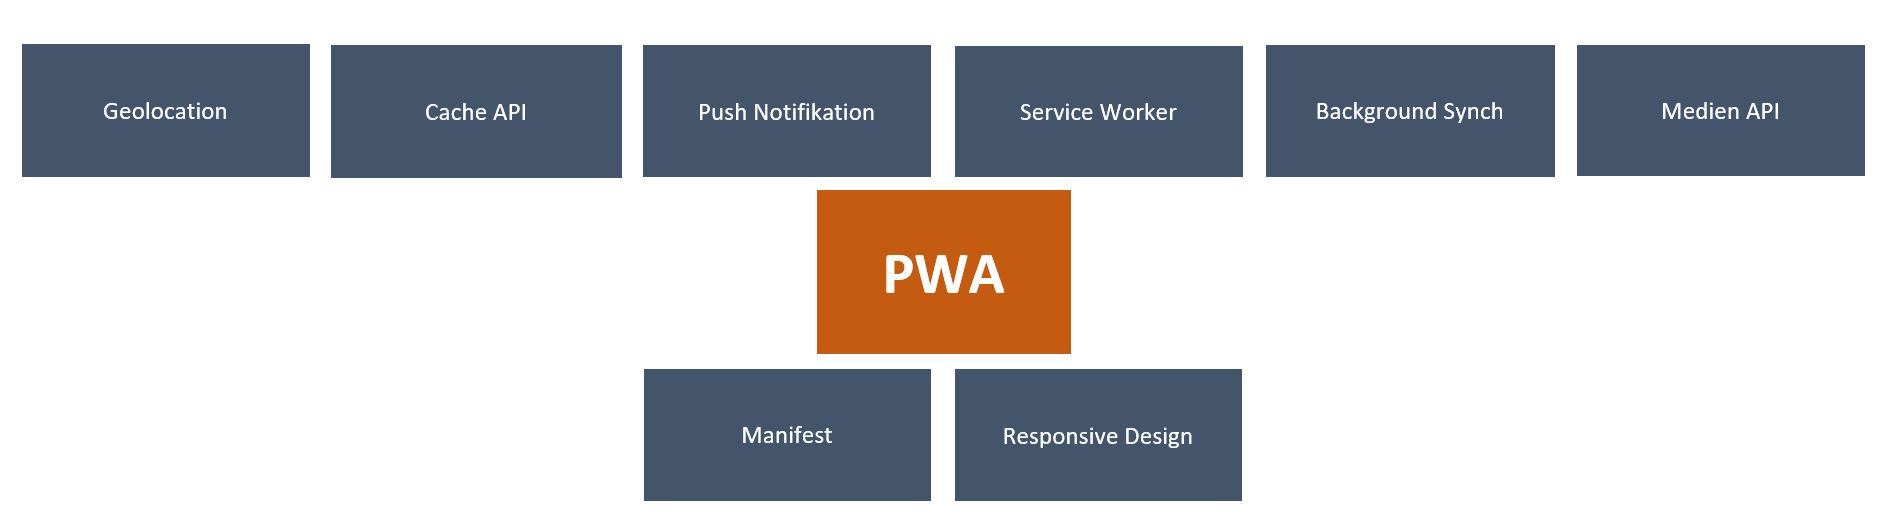
\includegraphics[width=14cm]{BilderAllgemein/PWA_Features}\medskip
	\caption{PWA Komponenten}
	\label{fig:Komponenten}
\end{figure}

\subsection{Tabelle}


%Tabelle verwenden





\section{Web App Manifest}
Das App Manifest ist ein JSON File verrät dem Browser wie sich die \acs{WA}, bei der Installation auf dem Startbildschirm, verhält. Im Manifest wird der Name,der Kurzname, die Größe, Aussehen der Icons und weitere Eigenschaften definiert diese im Kapitel \ref{chap:Entwurf} näher erklärt werden.

\subsection{Bereitstellung des Web App Manifest}
das App Manifest.json file wird in die gleiche Ebene wie die Index.html Datei in das Projekt eingepflegt und und übre den folgenden Link-Tag in der Index Datei bereitgestellt:


\begin{lstlisting}[language=HTML, caption={Manifest.json},label=lst:Manifest.json, xleftmargin=50pt]
<link rel="manifest" href="/<Dateinname>">
\end{lstlisting}

Der Aufbau der Manifest ist wie in Listening (Nr) gezeigt aufgebaut:







\cite{Manifest}


\section{Service Worker}
%\label{sec:Service Worker} zuweisung zu anderen Sektor
Der \acl{SW} (\acs{SW}) ist ein Script das der Browser im Hintergrund ausführt \cite{RegistrierungServiceWorker}. Mit der Hilfe des \acs{SW} ist es möglich die \acs{WA} offline zu betreiben, Push Notifikation zu erhalten, gecachte Daten abzurufen. \acs{SW} verhalten sich wie Proxy-Server, welche in einer Zwischenschicht vom Browser und den Netzwerk sitzen. 
Ein \acs{SW} wird von einem Worker-Kontext \cite{Worker} ausgeführt, hat keinen DOM Zugriff und wird als Haupt-Java Script Thread verwendet \cite{ServiceWorker}.

\subsection{Basis Architektur}
Der Cyclus eines \acs{SW}s ist von der Webseite getrennt.
In der Installationsphase werden benötigte statische Datein zwischengespeichert erst danach ist der \acs{SW} installiert. Die Installation erfolgt über die JavaScript-Funktion:

\begin{lstlisting}[language=JavaScript, caption={Service Worker Navigator},label=lst:ServiceWorkerNavigator, xleftmargin=50pt]
navigator.serviceWorker.register
\end{lstlisting}

Danach folgt die Aktivierungsphase, in dieser Phase werden alte Cache-Inhalte verwaltet und Aktualisiert.


\begin{figure}[h]
	\centering
	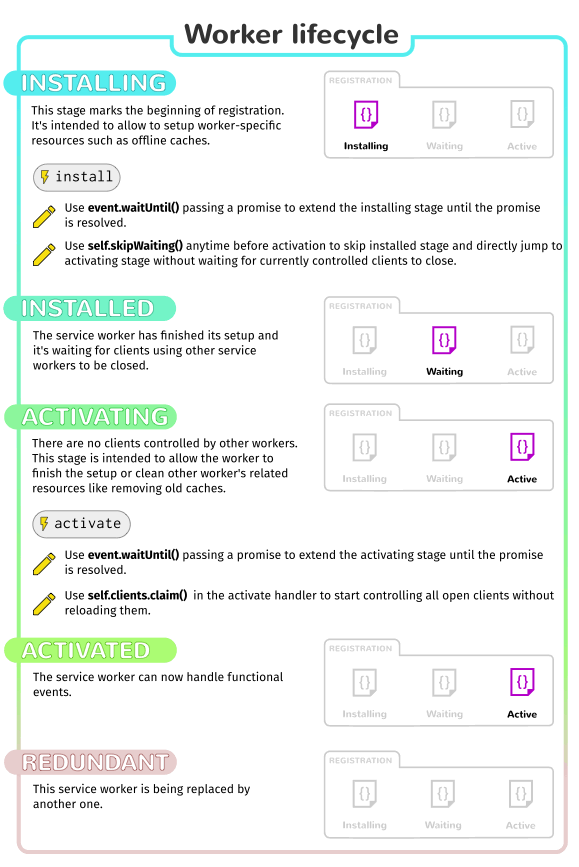
\includegraphics[width=8cm]{BilderAllgemein/swLifecycle}\medskip
	\caption{Basis Architektur \acl{SW}}
	\label{fig:Erstinstallation}\cite{ServiceWorkerArchitecture}
\end{figure}
Um die neuen Seiten zu steuern muss der \acs{SW} erneut geladen werden.
In der Abbildung \ref{fig:Erstinstallation} ist eine vereinfachte Erstinstallation zu sehen:

\subsection{Registrierung Service Worker}

Um den \acs{SW} zu registrieren muss folgender \acs{JS}-Code in das Projekt im (genauen Pfad rausfinden) integriert werden.
\begin{lstlisting}[language=JavaScript, caption={Service Worker Register},label=lst:ServiceWorkerRegister, xleftmargin=50pt]
if ('serviceWorker' in navigator) {
  window.addEventListener('load', function() {
    navigator.serviceWorker.register('/sw.js').then(function(registration) {
      // Registration was successful
      console.log('ServiceWorker registration successful with scope: ', registration.scope);
    }, function(err) {
      // registration failed :(
      console.log('ServiceWorker registration failed: ', err);
    });
  });
}
\end{lstlisting}

Hier wird die Unterstützung durch den Browser geprüft.

\begin{figure}[h]
	\centering
	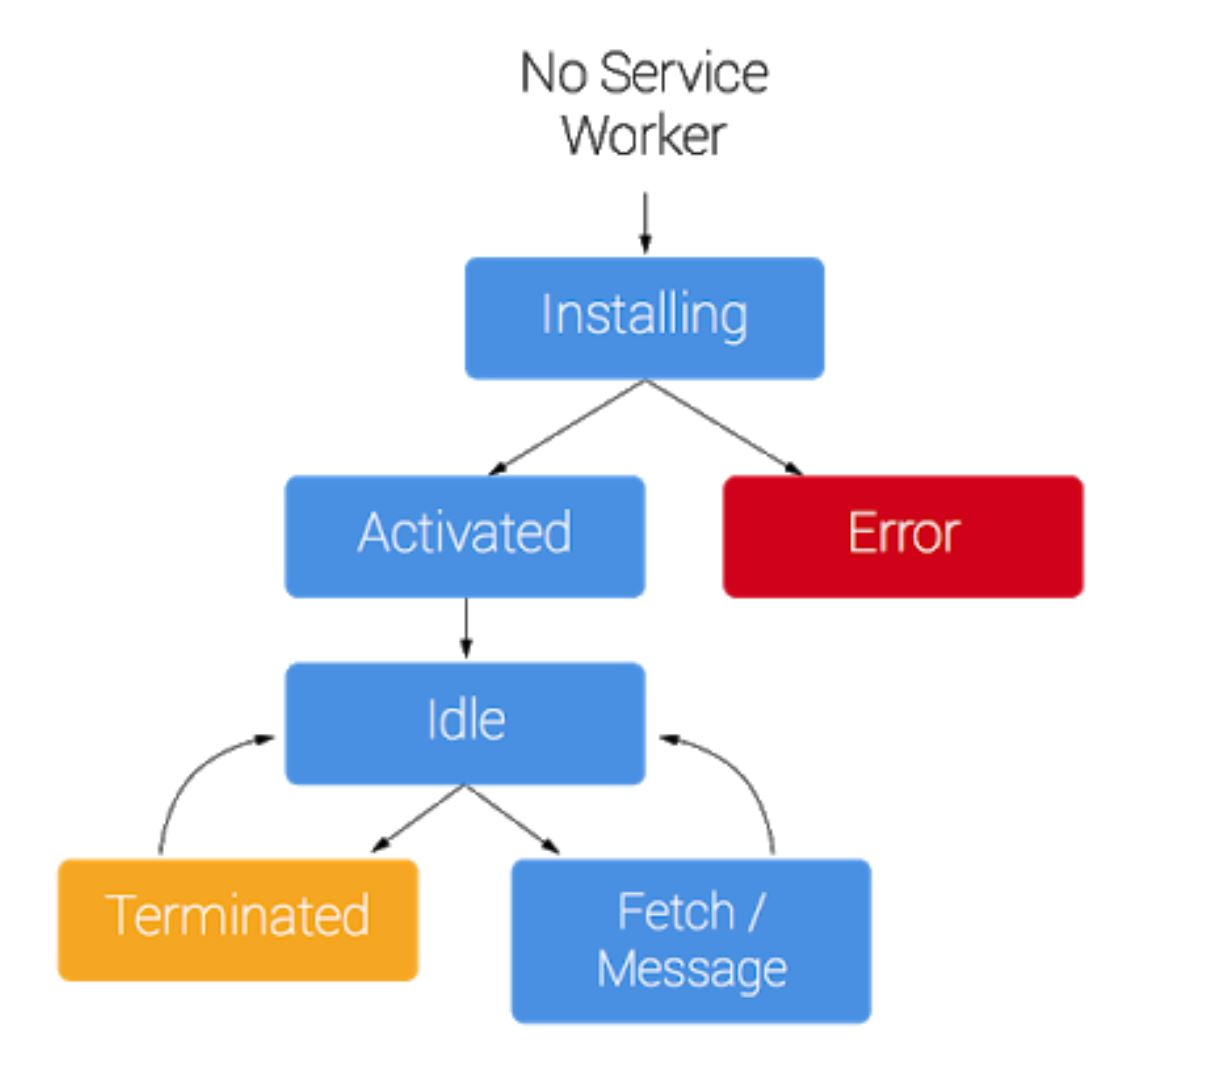
\includegraphics[width=14cm]{BilderAllgemein/InstallSW}\medskip
	\caption{Erstinstallation Service Worker}
	\label{fig:Erstinstallation}\cite{ServiceWorkerRegistration}
\end{figure}

Der \acs{SW} kann nach der Übernahme der Steuerung zwei Zustände übernehmen, entweder dieser wird beendet oder er übernimmt die Verwaltung der Netzwerkanfragen und der Nachrichten \cite{ServiceWorkerRegistration}.

\newpage

\section{Push Notifikation}
Um dem User bei einer \acs{PWA} das Gefühl einer Native App aufkommen zu lassen ist die Push Funktion unablässig. Erst durch diese Funktion in Kombination mit dem \acs{SW} gibt der \acl{WA} die persönliche Nähe zum User \cite{PushNotifikation}.


\subsection{Registrierung Push Notifikation}
Um die Push Funktion zu integrieren muss die Registerfunktion des \acs{SW} wie folgt erweitert werden:
 
\begin{lstlisting}[language=JavaScript, caption={Push Notifications},label=lst:PushNotifikation, xleftmargin=50pt]

if ('serviceWorker' in navigator && 'PushManager' in window) {
  console.log('Service Worker and Push is supported');

  navigator.serviceWorker.register('sw.js')
  .then(function(swReg) {
    console.log('Service Worker is registered', swReg);

    swRegistration = swReg;
  })
  .catch(function(error) {
    console.error('Service Worker Error', error);
  });
} else {
  console.warn('Push messaging is not supported');
  pushButton.textContent = 'Push Not Supported';
}
\end{lstlisting}


Hier wird der Support der Pushfunktionen durch den Browser überprüft wie in Kapitel \ref{chap:RegistrierungServiceWorker} die Browserunterstützung vom\acs{SW} und die Push Benachrichtigung. Bei fehlerlosen Durchlauf wird die \acs{SW}.js Datei registriert \cite{PushNotifikation}.

\newpage
\subsection{Cache API}

\subsection{Geolocation}
https://appdevelopermagazine.com/5877/2018/3/1/progressive-web-apps-vs-native-apps:-showdown-in-2018/


\subsection{Camera API}


\subsection{Browser} 


%\chapter{Entwurf}
\thispagestyle{standard}
\pagestyle{standard}
\renewcommand{\footrulewidth}{0.4pt}
\lfoot{\small Refik Kerimi}

In diesem Kapitel werden die Muster und die Anforderungen bzw. die Umsetzung der \acl{PWA}en (\acs{PWA}) im Allgemeinen betrachtet.


\section{Übersicht PWA}\label{sub:Übersicht PWA}
%https://developers.google.com/web/ilt/pwa/introduction-to-progressive-web-app-architectures
% Die Architektur soll beschrieben weden
Im Gegensatz zur \acl{NA} (\acs{NA}) ist die \acl{PWA} (\acs{PWA}) eine \acl{SC} (\acs{SC}) Architektur, diese wird nicht auf dem Client gespeichert sondern es wird über den Browser und das HTTPS-Protokoll zwischen Client und Server kommuniziert. Im Unterschied zu HTTP ist, wie in Abbildung \ref{fig:HTTP_HTTPS} zu sehen, die Verbindung verschlüsselt.

\begin{figure}[h]
	\centering
	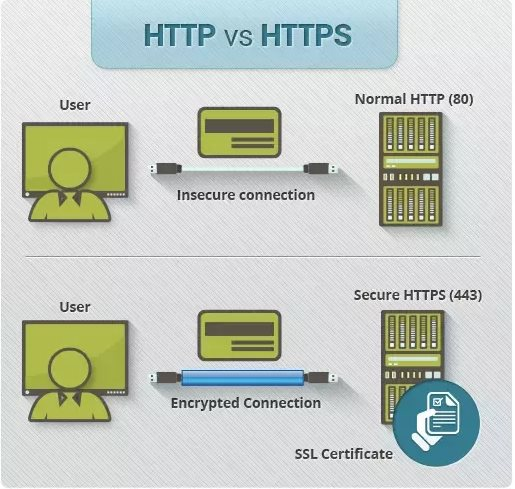
\includegraphics[width=6cm]{BilderAllgemein/HTTP_HTTPS}\medskip
	\caption{Unterschied HTTP/HTTPS \cite{HTTPS}}
	\label{fig:HTTP_HTTPS}
\end{figure}

Dies hat den Vorteil das die Applikation sowie die Updates wie schon in Kapitel \ref{chap:PWAvs.NativeApplikationvsWeb Applikation} erwähnt nicht downgeloaded und installiert werden müssen, das wird alles Server seitig erledigt. 

\newpage





\chapter{Implementierung}\label{chap:Implementierung}
\thispagestyle{standard}
\pagestyle{standard}
\lfoot{\small Refik Kerimi}

\section{Umsetzung der Anforderungen}\label{sub:Umsetzung der Anforderungen}
In diesem Kapitel wird die Umsetzung der Applikation beschrieben. Die Anforderungen aus Kapitel \ref{sub:Anforderungsanalyse}
Zur Erstellung des User Interfaces wird ReactJS\footnote{https://reactjs.org/docs/getting-started.html} und als CSS Framework Semantic-UI\footnote{https://react.semantic-ui.com/introduction} verwendet, Sematic-UI soll sicherstellen das die Applikation responives verhalten aufweist und für alle Bildschirmgrößen geeignet ist. Um die Daten zu versenden, aufzurufen und zu speichern wurde das JSON Key/Value Format, die Fetch API und der Browser Cache verwendet.
Als Browser wurde der Google Chrome Version 67 verwendet.
Die nicht fertigen Funktionen wurden mit Mockups dargestellt um einen Eindruck zu vermitteln wie das ganze in Zukunft aussehen wird.

\section{Ausgewählte Programmiersprache und IDE}
Als Programmiersprache wurde \acl{JS} (\acs{JS}) ausgewählt. 
Als Entwicklungsumgebung wurde Webstorm (Version) von Jetbrains verwendet. 
Weitere verwendete Tools und Frameworks wurden im Kapitel \ref{sub:Umsetzung der Anforderungen} beschrieben.


\section{Manifest}
\subsection{Aufbau}
\subsection{Implementierung}



\section{Service Worker und Cache API}

%\lstset{language=Java}
%\begin{lstlisting}[caption={Status},label=lst:Status, xleftmargin=50pt]
%public enum Status {
%	Nothing,
%	Error,
%	WertGeschrieben,
%	WertEmpfangen,
%	KeineVerbindungsparameter,
%	KeinGueltigerDatentyp
%}
%\end{lstlisting}

caching Files --> we´lche Files sollen gachaed werden
	1. Appshell --> statisch
		2.Style, Icons, Bilder
		3. nicht zu Viel chachen
		
		
Notizen Video
	Asynchronus Code Abschitt 6 Lektion 62 4:34 
	 

\subsection{Aufbau Offline Mode}
\subsection{Implementierung}

\section{Push Notifications}
\subsection{Aufbau}
\subsection{Implementierung}

\section{Geolocation API}
\subsection{Aufbau}
\subsection{Implementierung}











\chapter{Funktionstest/Validierung}\label{chap:Funktionstest}
\thispagestyle{standard}
\pagestyle{standard}
\lfoot{\small Refik Kerimi}

\section{Ausgangsbedingung und Ausgrenzung}
Getestet wurden die in Kapitel \ref{chab:Basistechnologien} und \ref{chap:Implementierung} beschriebenen PWA-Features. Dies wurde zum einen über die DevTools vom Chrome Browser sowie über das Chrome PlugIN Lighthouse getestet. 
Als mobiles Testgerät wurde das Nexus X5 mit der Android 8.1.0 Software verwendet.  
Weiters kann der Emulator von Android Studio verwendet werden um den Test ohne Androidgerät darzustellen. Die Applikation selbst wurde hier nicht behandelt.
 
\section{Testen auf Mobilen Geräten und Android Studio Emulator}
Um auf auf dem Mobilen Smartphone testen zu können muss der Developer Modus auf dem Gerät eingeschaltet werden. Dies wird durch das Aktivieren der Entwicklertools und das Freischalten der USB-Debugging Funktion wie in Abbildung \ref{fig:DevToolsAndorid} und \ref{fig:DevToolsChrome} zu sehen ist erreicht. 

\begin{figure}[h]
	\centering
	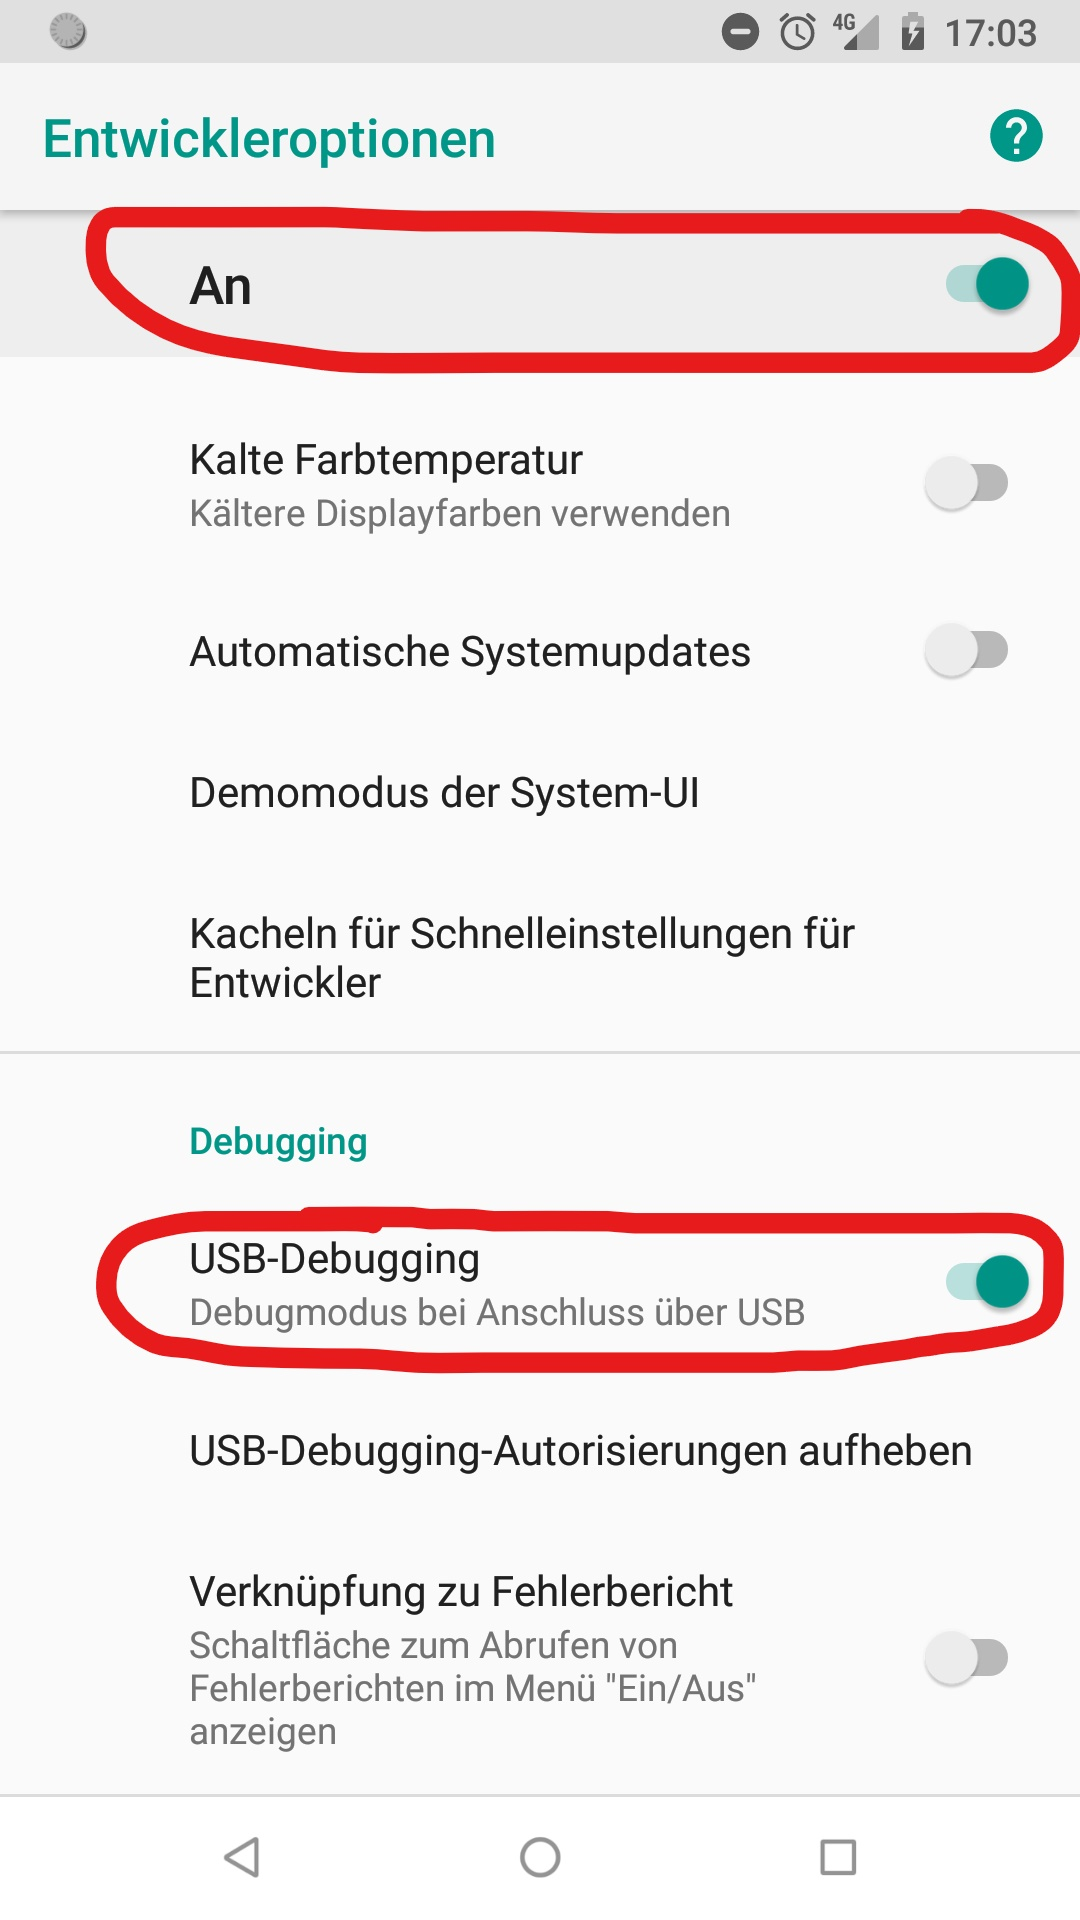
\includegraphics[width=6cm]{BilderAllgemein/DevToolsAndroid}\medskip
	\caption{Aktivieren der Entwicklertools auf Android 8.1.0}
	\label{fig:DevToolsAndorid}
\end{figure}

\begin{figure}[h]
	\centering
	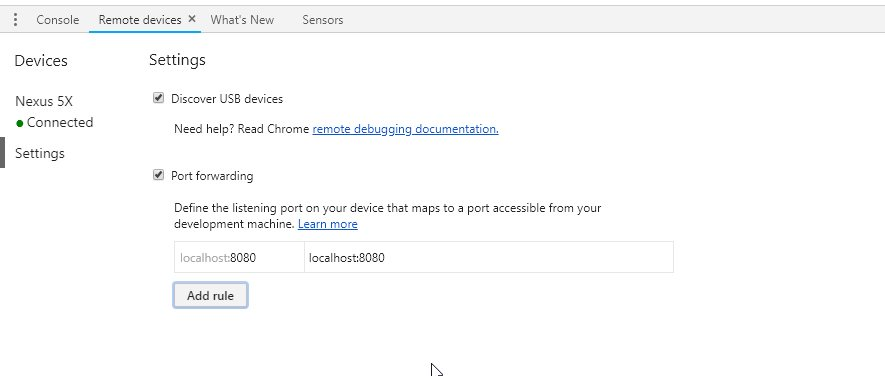
\includegraphics[width=14cm]{BilderAllgemein/DevToolsChrome}\medskip
	\caption{Anzeige der Verbindung auf Google Chrome 67}
	\label{fig:DevToolsChrome}
\end{figure}
\newpage
Falls kein Android Gerät zur Verfügung steht ist der von Android Studio\footnote{https://developer.android.com/studio/} angebotene Emulator eine große Hilfe. Durch den integrierten Emulator lassen sich verschiedene Softwareversionen von Android darstellen. Sie helfen bei der Entwicklung und beim Testen der \acs{PWA}.
\newpage
\section{Lighthouse}
Lighthouse ist ein open-source Tool von Google und unterstützt den Entwickler bei der Verbesserung und Transformation der Applikation zu einer vollwertigen \acs{PWA}. Man kann Lighthouse über 3 Wege verwenden:
\begin{itemize}
    \item  in Chrome DevTools
	\item  über die Kommandozeile
	\item  oder im Continues Integration Prozess als Node Module
\end{itemize}
Jeder dieser Workflows benötigt den Google Chrome Browser \cite{Lighthouse}.
Der Einsatz von Lighthouse über den Browser ist einfach. Nach eingabe der URL kann das Tool über das Chrome PlugIn, wie in Abbildung \ref{fig:LighthousePlugIN} zu sehen ist, gestartet werden. Lighthouse führt einen Debuggingtest (Abbildung \ref{fig:LighthouseDebugging}) aus und erstellt einen Bericht. In Abbildung \ref{fig:LightH_beforHTTPS_Overview} ist der Überblick der Applikation zu sehen und in Abbildung \ref{fig:PWA_Test_Lighthouse_noHTTPS} werden die fehlenden PWA-Features angezeigt.

\begin{figure}[h]
	\centering
	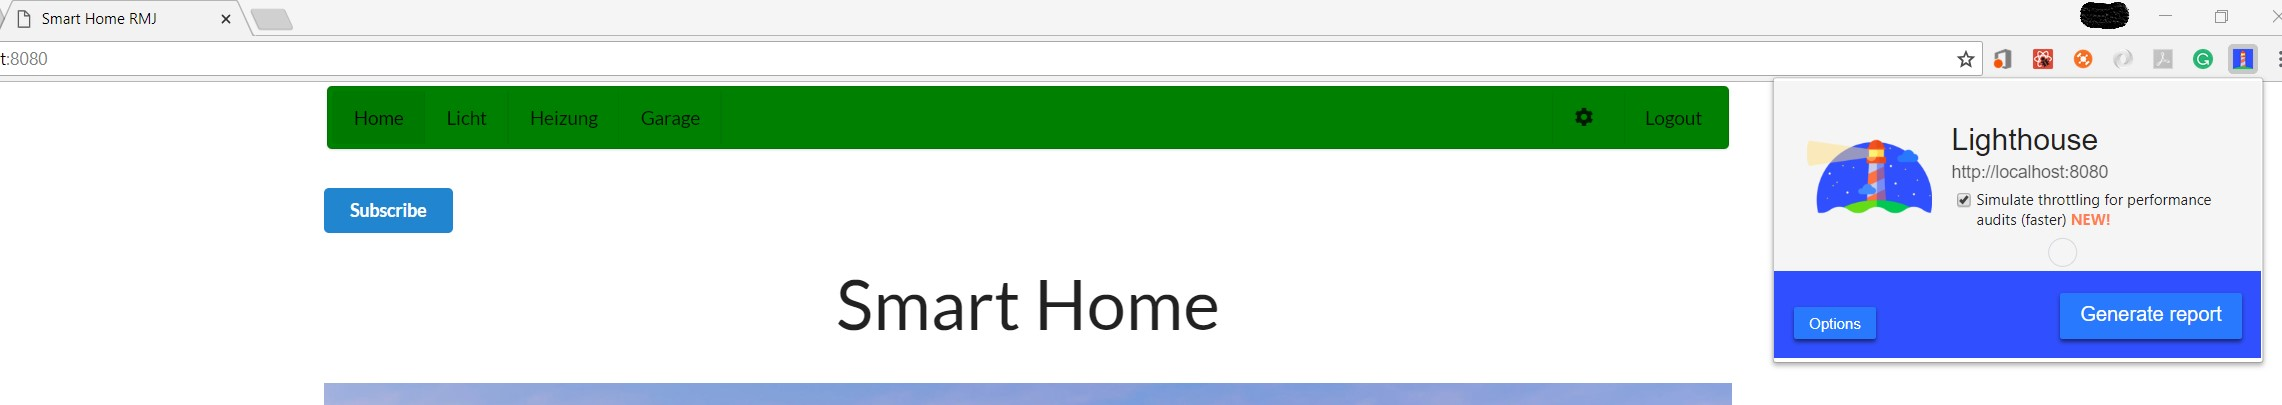
\includegraphics[width=6cm]{BilderAllgemein/Test/LighthousePlugIN}\medskip
	\caption{Lighthouse Plugin Chrome 67 }
	\label{fig:LighthousePlugIN}
\end{figure}
\begin{figure}[h]
	\centering
	
\includegraphics[width=6cm]{BilderAllgemein/Test/debuggingLighthouse}\medskip
	\caption{Debugging}
	\label{fig:LighthouseDebugging}
\end{figure}
 

\begin{figure}[h]
	\centering
	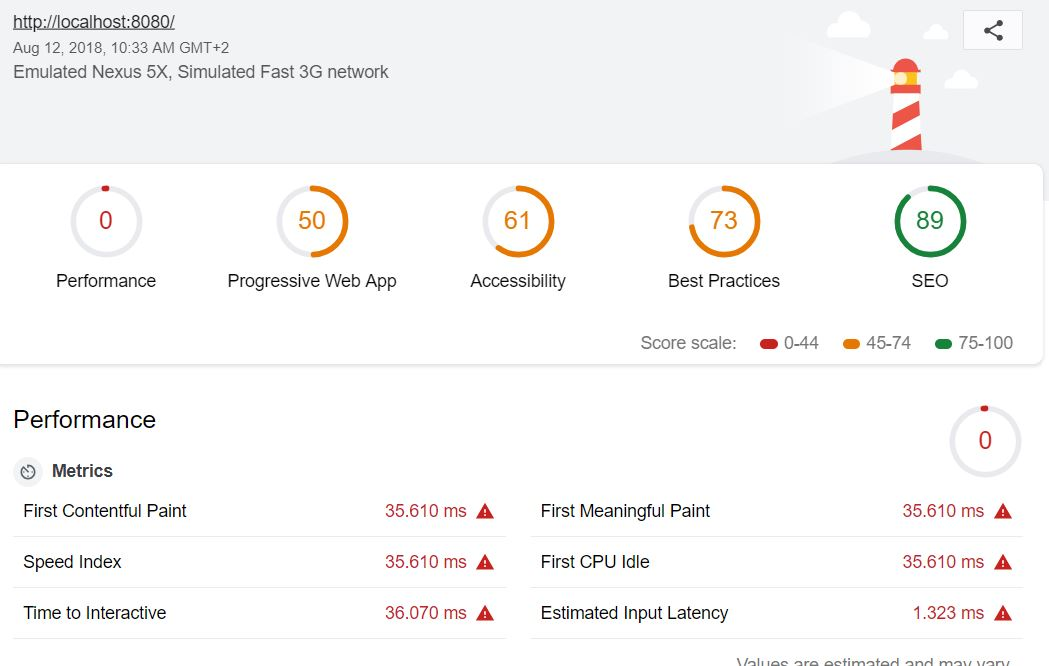
\includegraphics[width=8cm]{BilderAllgemein/Test/LightH_beforHTTPS_Overview}\medskip
	\caption{Lighthouse Überblick}
	\label{fig:LightH_beforHTTPS_Overview}
\end{figure}

\begin{figure}[h]
	\centering
	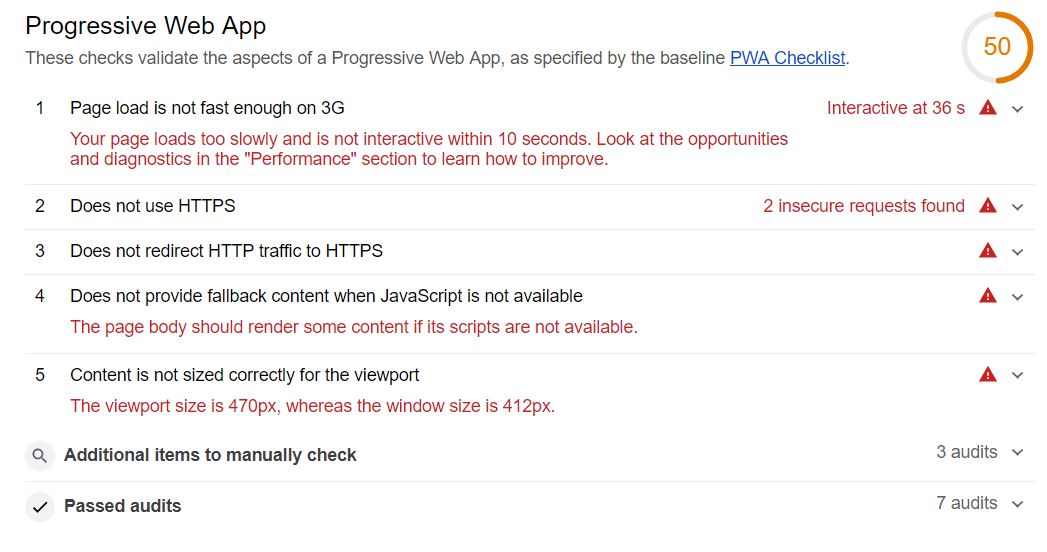
\includegraphics[width=10cm]{BilderAllgemein/Test/PWA_Test_Lighthouse_noHTTPS}\medskip
	\caption{Lighthouse fehlende PWA-Features}
	\label{fig:PWA_Test_Lighthouse_noHTTPS}
\end{figure}

In beiden Bericht Abbildungen erkennt man, dass die Applikation nur zur Hälfte die PWA Features enthält.
Dies kommt daher, weil die \acs{PWA} bei diesem Test auf auf dem Localhost läuft und nicht wie von Google gefordert über das HTTPS-Protokoll.
Das Projekt wurde für diese Arbeit nicht Live gestellt.

\newpage
\section{Add to Homescreen}
%https://developers.google.com/web/fundamentals/app-install-banners/#test
Durch dieses Feature sollte die \acs{PWA} dem Benutzer das Gefühl einer Nativen App geben. Doch leider funktioniert diese Funktion nicht immer wie sie sollte.
Das Feature ist zurzeit nur auf Android und Chrome Browsern verfügbar und ist damit weit entfernt von den Native Apps. Startet oft nicht automatisch, ist aber durch das Menu aufrufbar wie in Abbildung \ref{fig:} zu sehen ist.

\begin{figure}[h]
	\centering
	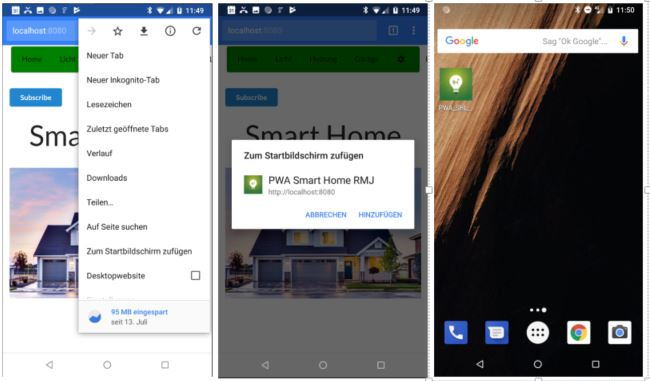
\includegraphics[width=10cm]{BilderAllgemein/Test/ADDHome}\medskip
	\caption{Add to Homescreen}
	\label{fig:ADDHome}
\end{figure}
\newpage

\section{Service Worker}
Die Status des Service Workers wird durch die DevTools geprüft.
Wie in Abbildung \ref{fig:SWTest} gezeigt ist pro \acs{PWA} nur ein Service Worker aktiv bei drei offenen Tabs. 

\begin{figure}[h]
	\centering
	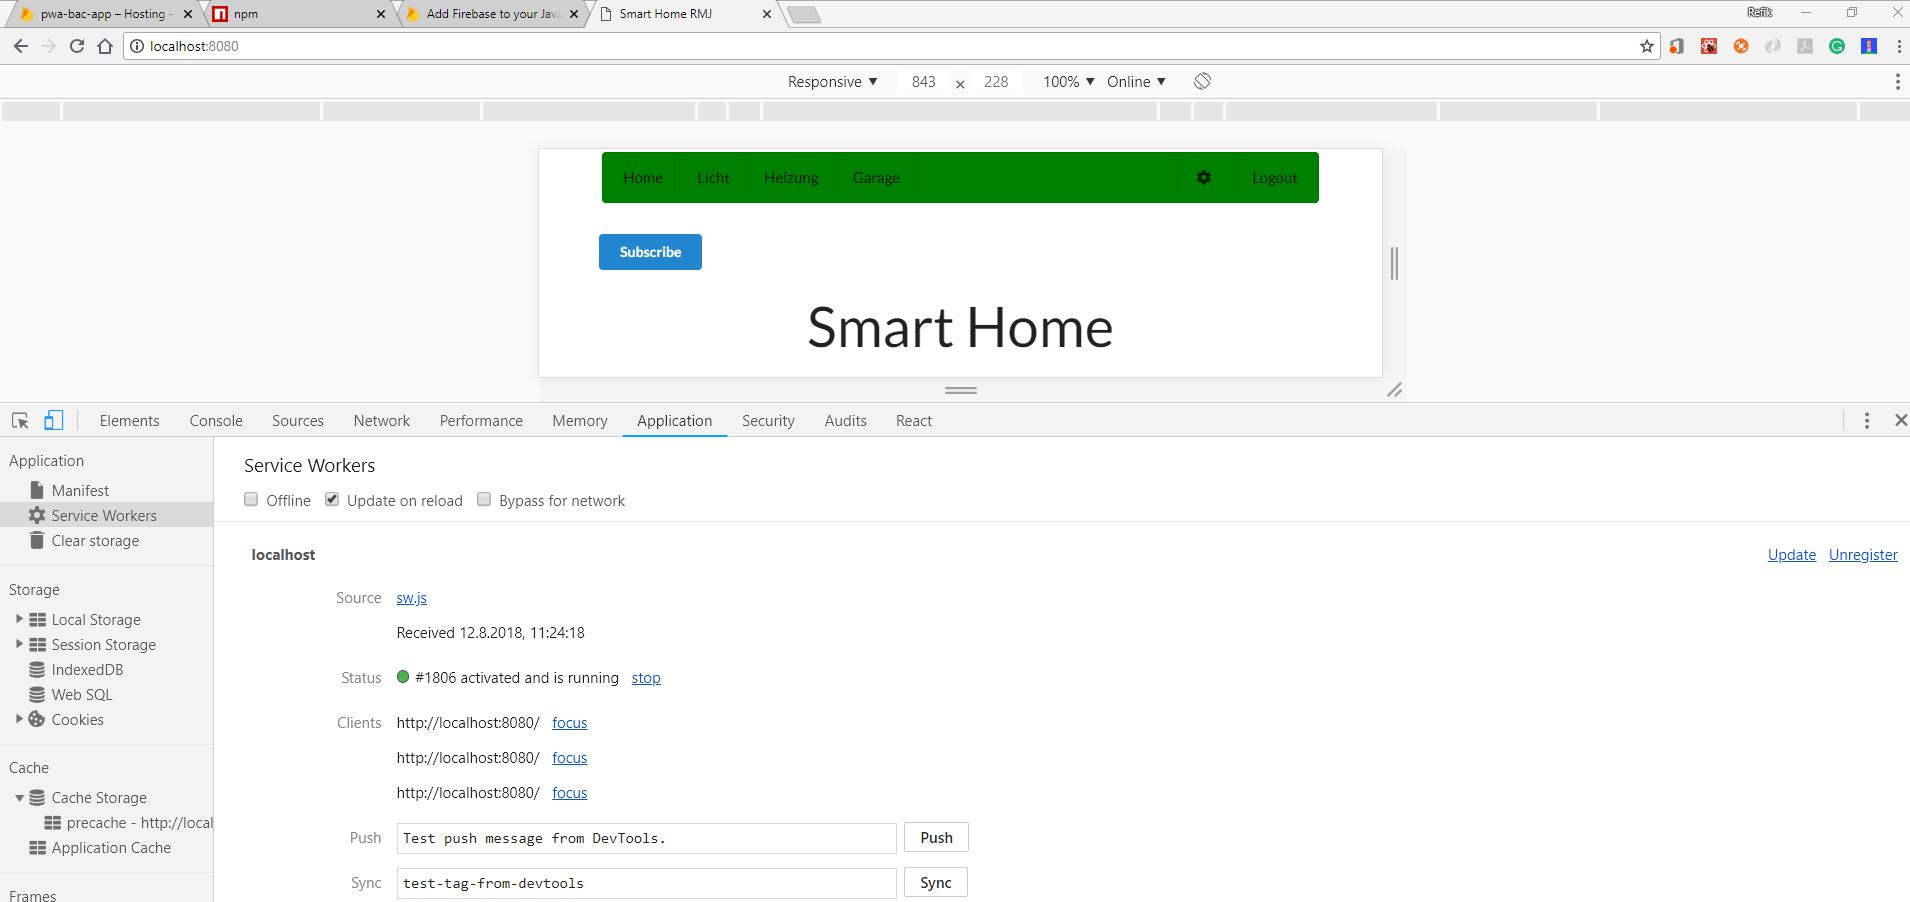
\includegraphics[width=10cm]{BilderAllgemein/Test/SW}\medskip
	\caption{Service Worker Status}
	\label{fig:SWTest}
\end{figure}
Weiters wurde die Offline Funktion der App getestet.
Abbildung \ref{fig:Offline} zeigt, dass die Applikation offline funktioniert.

\begin{figure}[h]
	\centering
	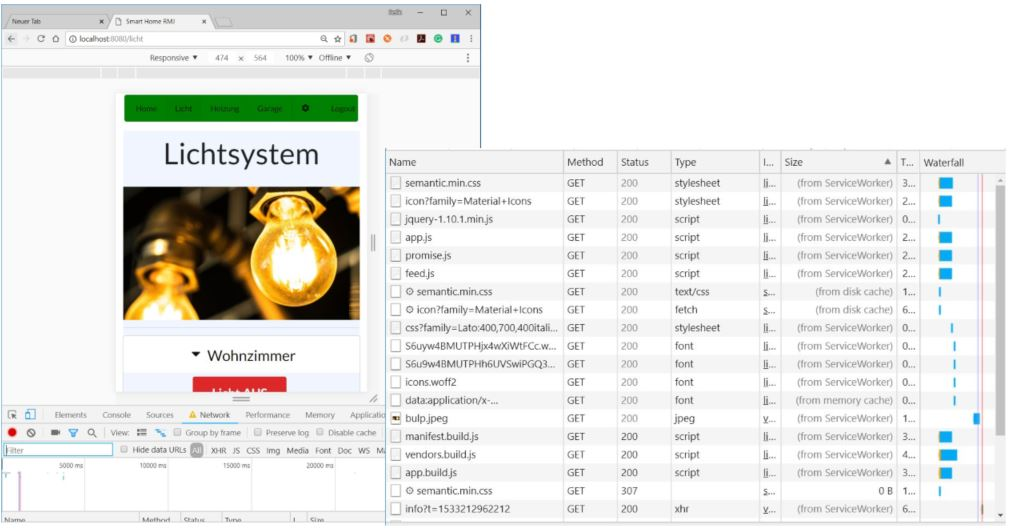
\includegraphics[width=14cm]{BilderAllgemein/Offline}\medskip
	\caption{Offline}
	\label{fig:Offline}
\end{figure}

\newpage

\section{Push Notifikation}
Um die Nachrichten erhalten zu können wird die Berechtigung (Abbildung \ref{fig:Registrierung}) als Erstes abgefragt und dann werden die Benachrichtigungen an den User erst verschickt siehe Abbildung \ref{fig:PushNotification}.

\begin{figure}[h]
	\centering
	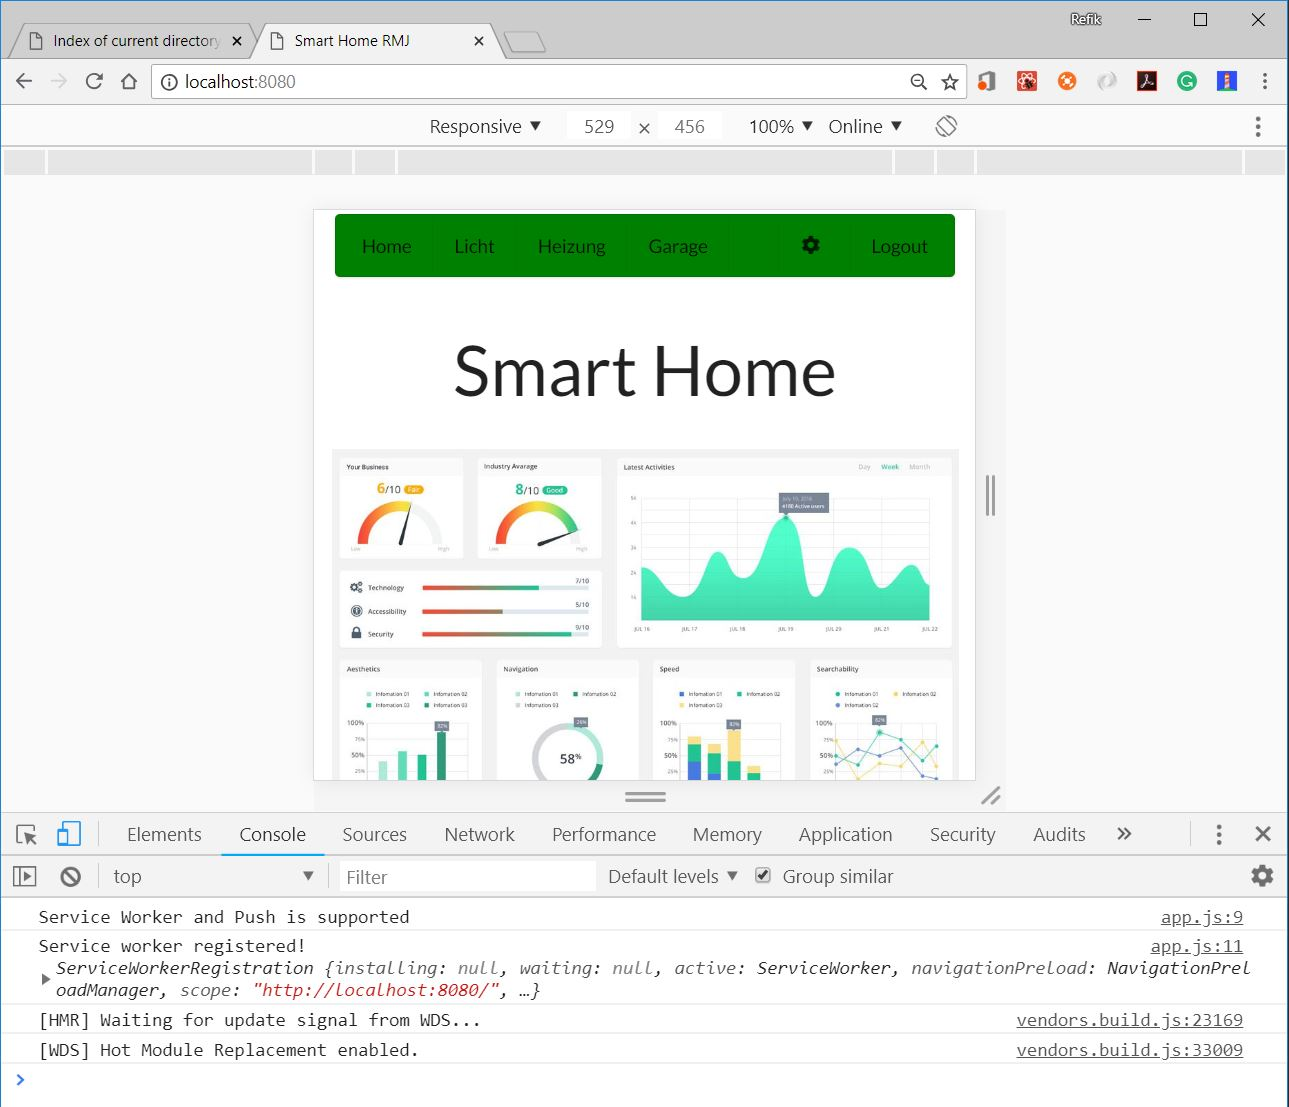
\includegraphics[width=10cm]{BilderAllgemein/PushNotification/Registrierung}\medskip
	\caption{Registrierung Push Notification}
	\label{fig:Registrierung}
\end{figure}

\begin{figure}[h]
	\centering
	
\includegraphics[width=14cm]{BilderAllgemein/PushNotification/Nachricht}\medskip
	\caption{Push Notification}
	\label{fig:Nachricht}
\end{figure}


\section{Geolocation}
Die Geolocation Funktion muss den Nutzer immer fragen ob dieser seinen Standort bestimmt haben will. Wie in Abbildung \ref{fig:Registrierung} zu sehen ist, wird das in dem Prototypen umgesetzt. In der Abbildung \ref{fig:Maps} sieht man wie der Standort über die Geolocation-API ermittelt worden ist.

\begin{figure}[h]
	\centering
	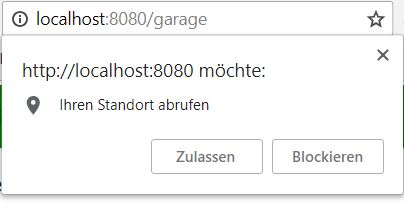
\includegraphics[width=10cm]{BilderAllgemein/Geolocation/Registrierung}\medskip
	\caption{Registrierung Geolocation}
	\label{fig:Registrierung}
\end{figure}

\begin{figure}[h]
	\centering
	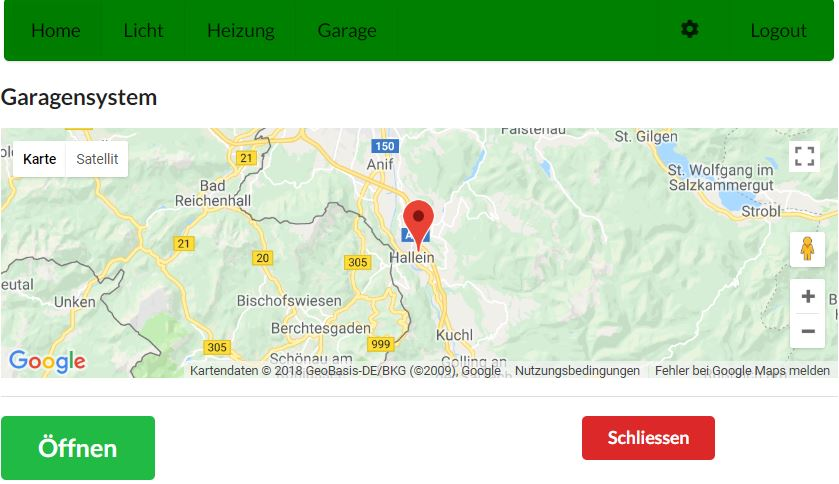
\includegraphics[width=14cm]{BilderAllgemein/Geolocation/Maps}\medskip
	\caption{Standortermittlung}
	\label{fig:Maps}
\end{figure}


\section{Vergleich mit native App}
Im Vergleich zur Nativen App bietet die \acs{PWA} einige Vorteile 





\chapter{Zusammenfassung und Ausblick}
\thispagestyle{standard}
\pagestyle{standard}
\renewcommand{\footrulewidth}{0.4pt}
\lfoot{\small Refik Kerimi}

In diesem Projekt hat sich gezeigt, dass die \acs{PWA} die nativen Applikationen nicht zur Gänze ablösen kann. Es ist sicherlich so, dass die \acs{PWA} eine Verbesserung der \acs{Web-App}s darstellt, aber sie arbeitet trotzdem nicht so gut wie eine für das Betriebssystem konzipierte Applikation.
Probleme gab es beim offline Arbeiten durch die Verwendung des \acs{JS}-Frameworks ReactJS. Durch die modulare Bauweise wurden die gecachten Files nicht immer richtig geladen und es ist mehr oder weniger Zufall, ob die Offlinefunktion tatsächlich wie gewünscht läuft. Doch auch wenn diese Funktion optimierungsbedürftig ist, stellt sie eine Verbesserung der Applikation dar, da bei geringer Internetgeschwindigkeit die App trotzdem sehr schnell und flüssig funktioniert. Bei der Entwicklung mit \acs{HTML}5, \acs{CSS} und \acs{JS} sollte es besser funktionieren. Dies wurde in dieser Arbeit aber nicht behandelt. 
Der Service Worker ist sehr einfach zu implementieren und arbeitet ohne irgendwelche Behinderungen im Hintergrund.
Die Push Notifikation ist eine große Bereicherung für die Browserapplikation, da dadurch Apps wie z.B.: Smart Home Apps, Sozial Media Apps, uvm. die User viel besser erreichen können. Durch das Hinzufügen des Icons auf dem Startbildschirm wird zusätzlich eine höhere Kundenbindung erreicht. Der Vorteil dabei ist, dass der Kunde nicht mehr über den Browser durch die Eingabe der URL auf die Webseite gelangt, sondern über seinen Startbildschirm wie bei einer nativen Applikation. Ein Nachteil ist sicherlich die Browserkompatibilität. Die \acs{PWA} wird nicht von allen Herstellern unterstützt und einige Features sind nur auf Android Geräten verfügbar. 
\\Im großen und ganzen ist die \acs{PWA} eine sehr aufregende Form der \acs{Web-App}s und man wird in Zukunft noch einiges davon hören.
Als ich diese Arbeit Anfang des Jahres begann, war die Community noch sehr klein. Doch innerhalb von ein paar Monaten hat sie sich verändert und ist sehr gewachsen. Es finden sich viele nützliche Tipps online, die es ermöglichen in sehr kurzer Zeit aus einer bestehenden App eine \acs{PWA} zu erstellen. 
%\chapter{Einleitung}

\thispagestyle{standard}
\pagestyle{standard}
\section{Motivation}

Die zunehmende Vernetzung und die immer stärkere Integration von Systemen macht
auch vor dem Bereich der Automatisierungstechnik nicht Halt. So ist hier in den letzten
Jahren ein steigender Bedarf an Interkonnektivität der einzelnen, vormals autonomen
Systeme zu verzeichnen. Vorschub leistet dieser Bewegung, dass durch die gestiegene
Verfügbarkeit von breitbandigen Verbindungen auch der Wunsch nach höherer Integrationsdichte
gewachsen ist. Immobilien, Ladengeschäfte, Produktionsstätten oder ganze
Firmenstandorte werden zunehmend als Verwaltungseinheiten gesehen, für die eine Administration
und Überwachung aus der Ferne oder die Einbindung in Firmennetze erfolgen
soll.
Auch der immer häufigereWunsch, Geschäftsprozesse automatisiert in Software abzubilden,
lässt es sinnvoll erscheinen, auf verschiedene Systeme eines Standorts aus der Ferne
als Entität zugreifen zu können. Damit verändern sich auch die Anforderungen an die
Schnittstellen eines Systems. Waren früher systemindividuelle Bediener vor Ort für die
Betreuung ausreichend, so soll dies heute immer öfter auch aus der Ferne zentral über
eine standardisierte Schnittstelle möglich sein. Somit hält die Problematik der verteilten
Anwendungen auch in vormals oft vollständig unabhängigen Systemen Einzug.
Gerade in der Automatisierungstechnik macht sich bemerkbar, dass der scheinbare Wildwuchs
an konkurrierenden Bus Systemen der letzten Jahre zu einer extremen Inkompatibilität
der Systeme geführt hat. Systeme die nun wieder eine Einheit im Sinne der remoten
Verwaltung bilden sollen. An Hand der Energieverwaltung eines Gebäudes oder
einer Produktionsstätte lässt sich dies veranschaulichen. Für eine zentrale Überwachung



\section{Zielsetzung}

\section{Anmerkung}

\chapter{Grundlagen}

\section{OpenNES}

\subsection{Architektur}

\subsection{}

\section{ModBus Protokoll}

\section{Abbildungen}

In Moby-Dick geht es in erster Linie um die Jagd auf einen weißen Pottwal \footnote{nach: https://de.wikipedia.org/wiki/Moby-Dick}. Kurze Zitate (unter drei Zeilen) müssen mit Anführungszeichen gekennzeichnet werden. Außerdem müssen die Quelle sowie die Seite angegeben werden. Ein Beispiel für ein kurzes Zitat: \glqq Komisch. Manch einer von uns wünschte sich, er lebe auf einer Südseeinsel.\grqq \cite{MELVILLE:MOBYDICK1997} (Seite 100).

  \begin{quote}
"Das Buch hier Lieblingsbuch. Viele Blätter viele, schöne Bilder. Du kennen Worte?"\newline
"Ja"\newline
"Ich kennen Bilder. Das ein Wal. Du lesen Worte!"\newline
"Durch das Herz des Wals strömt mehr Flüssigkeit als durch das große Wasserleitungsrohr unter der London Bridge, jedoch strömt das Wasser nicht so stark, wie das Blut, das vom Herz des Wals pocht."\newline
"Du gut, ich danken dir."  \upshape \cite{MELVILLE:MOBYDICK1997} (Seite 500)
  \end{quote}

Ein sehr praktisches Package ist cleveref. Es automatisiert und erleichtert das setzen von Referenzen ungemein. Als Beispiel wird eine Referenz auf das FHS-Logo gesetzt siehe \cref{FIG_LOGO}.

Für das Verfassen von wissenschaftlichen Arbeiten können eine Vielzahl an Quellentypen herangezogen werden. Beispiele hierfür sind Leitfäden (Manuals) \citep{RFC2828} \citep{80211i} \citep{80211} \cite{X800} \citep{TR102377} \citep{EN301893} \citep{PUB197} \citep{PUB74}, Bücher \citep{Fis04a} \citep{Rei05a} \citep{Tan00a} \citep{Ste04a} \citep{GMS00a} \citep{HL98a}, Sammelbände \citep{EHL00a} \citep{Sch94a}, Journal-Artikel \citep{TM03a} \citep{CP03a}, Konferenz-Proceedings \citep{HCB00a} \citep{KBW04a} \citep{KSW04a} \citep{HK05a}, Internetmagazine \citep{Eke05a}, Webquellen \cite{nist} \cite{php} \cite{BDKMT93a} \cite{IDSSM} sowie Diplomarbeiten und Dissertationen \citep{Sch98} \cite{Hae94a}.

Als Beispiel für eine Abkürzung wird hier \ac{ADF} angeführt. Das Package schreibt automatisch das erste Vorkommen der Abkürzung aus. Die zweite Verwendung von \ac{ADF} wird also abgekürzt. Ist ein Ausschreiben einer Abkürzung gewünscht wird der acl-Befehl verwendet. Dies führt zu \acl{ADF}. Abkürzungen müssen in der Datei \glqq 05Abkuerzungsverzeichnis\grqq angegeben werden.

\section{Quelltext}

\texttt{printf("Hallo Welt")} für Ausschnitte von Sourcecode innerhalb von Text

\lstset{escapeinside={\%*}{*)},numbers=none}%oder numbers=left
\begin{lstlisting}[language=C,
caption=Beispiel-Listing,
label=LST_SAMPLE]
serverTCP = new TcpListener(IPAddress.Parse(serverIP), serverPort);
\end{lstlisting}

\lstset{escapeinside={\%*}{*)},numbers=left}
\lstinputlisting[language=Matlab, caption=Einfaches Matlabprogramm in einer Datei, label=list:hello.m]{Listings/hello.m}
\section{Text}

\section{Refik}

\section{Bilder}

\begin{figure}[H]
\begin{center}
	
\includegraphics[scale=0.4]{BilderAllgemein/Logo.jpg}
\end{center}
	%\includegraphics[width=\textwidth]
	%\end{center}
	% Title
	\caption{Das FHS-Logo}
	% Unique name: identifier for referencing
	\label{FIG_LOGO}
\end{figure}

\section{Formeln}

Formeln sind für jeden Abschnitt rechtsbündig von dieser zu nummerieren, um einen späteren Bezug in der Arbeit zu gewährleisten. Formeln werden üblicherweise in "`Computer Modern Roman"' (\LaTeX{}-Standard) gesetzt. In diesem Template wird die Formel-Schrift bzw. das Package \texttt{eulervm} verwendet. Abgesetzte Formeln werden in \LaTeX{} durch die 
\emph{equation} Umgebung definiert. Formelausdrücke innerhalb von Textabschnitten erhält man durch \$Formel\$.

\subsection*{Beispiel}
%
Der \emph{Sinus cardinalis} oder sinc-Funktion ist eine mathematische Funktion $f$, welche in nicht-normierter Version als

\begin{equation}
	f(x) := \frac{\sin(x)}{x}
	\label{eq:bsp}
\end{equation}

definiert wird. In der digitalen Signalverarbeitung findet meistens nachfolgende normierte Version $\mathrm{si}(x)$ oder $\mathrm{sinc}(x)$ Anwendung \cite{x1}, \cite{x2}. Für eine Visualisierung dieser Funktionen siehe Abb.~\ref{FIG_LOGO}.

\begin{equation}
	f(x) := \frac{\sin(\pi x)}{\pi x}
	\label{EQ_SAMPLE}
\end{equation}

\section{Beispiel für Tabellen}
%
Es empfiehlt sich, für Tabellen die Standard-\LaTeX{}-Umgebung \emph{tabular} zu verwenden. Bei Bedarf können natürlich auch Erweiterungen (z.B.~\emph{tabularx} oder \emph{array}) zur Anwendung kommen. Eine mögliche Darstellung zeigt Tabelle \ref{Table_Sinc}.

\begin{table}[h!]%
	\begin{center}
	
		\begin{tabular}{|r|r|r|}
			\firsthline
			$x$&$\mathrm{sinc}(x)$&$\mathrm{sin}(x)$\\\hline\hline
			$-0.5$&0.6366&-0.4794\\\hline
			$0$&1.0000&0\\\hline
			$0.5$&0.6366&0.4794\\\hline
		\end{tabular}
		\caption{Zwei Werte der Sinc-Funktion}
		\label{Table_Sinc}
	\end{center}
\end{table}













%%%%%%%%%%%%%%%%%%%%%%%%%%%%%%%%%%%%%%%%%%%%%%%%%%%%%%%%%%%%%%%%%%%%%%%%%%%%%%%%%%%%%%%%%%%%%%%%%%%%%%%%%%%%
% LITERATURVERZEICHNIS

\interlinepenalty = 10000 % Literatureinträge: Absätze zusammenhalten
\clearpage
\addcontentsline{toc}{chapter}{Literatur}
\singlespace
\raggedright
\bibliography{12Literatur}
\interlinepenalty = 100

%%%%%%%%%%%%%%%%%%%%%%%%%%%%%%%%%%%%%%%%%%%%%%%%%%%%%%%%%%%%%%%%%%%%%%%%%%%%%%%%%%%%%%%%%%%%%%%%%%%%%%%%%%%%
% ANHÄNGE

\begin{appendix}
%\include{Anhang_Mathematik}                 % A
%\include{Anhang_FormatDerParameterdateien}  % B
%\include{Anhang_Quelltexte}                 % C
%\include{Anhang_Datenblaetter}              % D
%\include{Anhang_Glossar}                    % E
\end{appendix}

\end{document}